\documentclass[11pt,a4paper]{article}
\usepackage{graphics}
\usepackage{alltt}
\usepackage[portuges]{babel}
\usepackage[utf8x]{inputenc}
\usepackage{color}
\usepackage{fancyhdr}
\usepackage{listings}
\usepackage{multicol}
\usepackage{babel}
\usepackage{hyperref}
\usepackage{t1enc}
\usepackage{aeguill}
\usepackage{varioref}
\usepackage{fancyvrb}
\usepackage{color}
\usepackage{cite}
\usepackage{float}
\usepackage{listings}
\usepackage{harvard}
\usepackage{geometry}
\usepackage{setspace}
\usepackage{thumbpdf}
\usepackage{fancyhdr}
\usepackage{lastpage}
\usepackage{alltt}
\usepackage{graphicx}
\usepackage{verbatim}
\usepackage{color}
\usepackage{url}
\usepackage{epsf}
\usepackage{listings}
\usepackage[refpages]{gloss}
\usepackage{array}
\usepackage{longtable}
\usepackage{multirow}
\usepackage{amsmath, amsthm, amssymb}
\usepackage{slashbox}
\usepackage{rotating}

\setlength{\textwidth}{16.5cm}
\setlength{\textheight}{24cm}
\setlength{\parindent}{1em}
\setlength{\parskip}{0pt plus 1pt}
\setlength{\oddsidemargin}{0cm}
\setlength{\evensidemargin}{0cm}
\setlength{\topmargin}{-1.1cm}
\setlength{\headsep}{20pt}
\setlength{\columnsep}{1.5pc}
\setlength\columnseprule{.4pt}
\setlength\premulticols{6\baselineskip}
\pagestyle{fancy}

\definecolor{castanho_ulisses}{rgb}{0.71,0.33,0.14}
\definecolor{gray_ulisses}{gray}{0.55}
\definecolor{green_ulises}{rgb}{0.2,0.75,0}

\lstdefinelanguage{C_ulisses}{
	basicstyle=\ttfamily\scriptsize,
    sensitive=true,
	morecomment=[l][\color{gray_ulisses}\scriptsize]{//},
	morecomment=[s][\color{gray_ulisses}\scriptsize]{/*}{*/},
	morestring=[b]",
	morestring=[b]',
	stringstyle=\color{red},
	showstringspaces=false,
	numbers=left,
	numberstyle=\tiny,
	numberblanklines=true,
	showspaces=false,
	showtabs=false,
	xleftmargin=-10pt,
	xrightmargin=-20pt,
	emph=
	{[1]
		return,printf,fprintf,if,else,scanf,sscanf,sprintf,malloc,
		calloc,realloc,fgets,fputs,puts,system,strcmp,strstr,
		strchr,exit,for,while,fclose,fopen,atoi,sizeof,sin,cos
	},
	emphstyle={[1]\color{blue}\textbf},
	emph={[2]char,float,double,void,NULL,int,bool},
	emphstyle={[2]\color{green_ulises}\textbf},
	emph={[3]typedef, struct},
	emphstyle={[3]\color{castanho_ulisses}\textbf}
}

\lstdefinelanguage{txt}
{
       basicstyle=\ttfamily\scriptsize,
       showstringspaces=false,
       numbers=left,
       numberstyle=\tiny,
       numberblanklines=true,
       showspaces=false,
       showtabs=false
}
\lstnewenvironment{code_txt}{\lstset{language=txt}}{}
\lstnewenvironment{code_c}{\lstset{language=C_ulisses}}{}

\lstnewenvironment{code_lex}
{\textbf{Código Lex} \hspace{1cm} \hrulefill \lstset{language=txt}}
{\hrule\smallskip}

\title{\sf  Engenharia de Linguagens \\ Engenharia Gramatical \\
\begin{tabular}{c}
    
\includegraphics[width=.1\textwidth]{stuff/uminho.jpg}
    
\includegraphics[width=.07\textwidth]{stuff/informatica.jpg}\\
    {\small Universidade do Minho}, {\small MEI}\\
    {\small Ano lectivo 2010/2011}\\
    {\small Trabalho Prático}\\
\end{tabular}
}
\author{
    {\small José Pedro Silva - pg17628} \and
    {\small Mário Ulisses Costa - pg15817} \and
    {\small Pedro Faria - pg17684}}
\date{{\small \today}}

\begin{document}
\maketitle

\begin{abstract}
Descrição da solução proposta para os problemas do dia 08-11-2010
\end{abstract}

\tableofcontents

\newpage
\section{Problema}

Considere a linguagem de programação Lisp na qual um programa é uma Symbolic-Expression (SExp). Sabe-se que uma SExp é um valor atómico (palavra ou numero) ou é uma lista e que cada elemento da lista é uma SExp.

A GIC abaixo define formalmente a linguagem Lisp, de acordo com a descrição acima: 

\begin{verbatim}
      T = { num, pal, "(", ")" }
      N = { Lisp, SExp, SExplist }
      S = Lisp
      P = {
            p1: Lisp     --> SExp
            p2: SExp     --> num
            p3: SExp     --> pal
            p4: SExp     --> "(" SExplist ")"
            p5: SExplist --> SExp SExplist
            p6: SExplist --> &
          }
\end{verbatim}

Pede-se então que escreva uma Gramática de Atributos, GA, para

\begin{itemize}
  \item a) calcular o nível de aninhamento de cada lista (comece em 1 para a lista principal).
  \item b) construir uma lista com todos os "operadores" presentes (considera-se "operador" o 1ºelemento de cada lista).
  \item c) verificar se todos os "operadores" usados pertencem ao conjunto de operadores válidos de acordo com uma "biblioteca" fornecida no inicio.
  \item d) verificar se o numero de argumentos ("operandos") com que cada operador é invocado condiz com a cardinalidade associada aos operadores válidos na referida "biblioteca".
\end{itemize}
\newpage
\section{Solução}
As subsecções que se seguem referem-se à resolução de cada alínea do capítulo anterior.

\subsection{Alínea a)}
A solução para a primeira alínea é a criação de um atributo herdado \emph{alinh} do tipo \emph{Integer} que ocorrerá nos Não Terminais \emph{SExp} e \emph{SExpList}, conforme se poderá ver no código seguinte: 

\begin{lstlisting}[frame=single, numbers=right, basicstyle=\tiny, caption={Code to a Contextual Condition for Symbol Transition}, label={lst_semantics}]
inherited attribute alinh :: Integer;
attribute alinh occurs on SExp, SExpList;
\end{lstlisting}

O valor será incrementado na produção \texttt{SExp --> "(" SExplist ")"} e adicionado ao atributo sintetizado \emph{output} para posteriormente ser imprimido para o ecrã (código em ~\ref{lst_semantics}).

\begin{lstlisting}[frame=single, numbers=right, basicstyle=\tiny, caption={Code to a Contextual Condition for Symbol Transition}, label={lst_semantics}]
concrete production sExp3
se::SExp ::= '(' sel::SExpList ')'
{se.output="["++ sel.output ++ ":"  ++ toString(se.alinh) ++ "]";
sel.alinh = se.alinh + 1;
}
\end{lstlisting}

\subsection{Alínea b)}

Para esta alínea, foram precisos dois atributos para a sua resolução. O primeiro, \emph{ishlista}, é um valor herdado booleano que será preciso para verificar se o valor a retirar é o primeiro da lista ou não. \\

Pela Figura~\ref{fig arv} podemos ver como esse atributo (que ocorre nos Não Terminais \emph{SExp} e \emph{SExpList}) será tratado. A figura representa a árvore de derivação (incompleta) para o exemplo \texttt{(add (add 1 2) (mul 3 4))}. \\

\begin{figure}[h]
\begin{center}
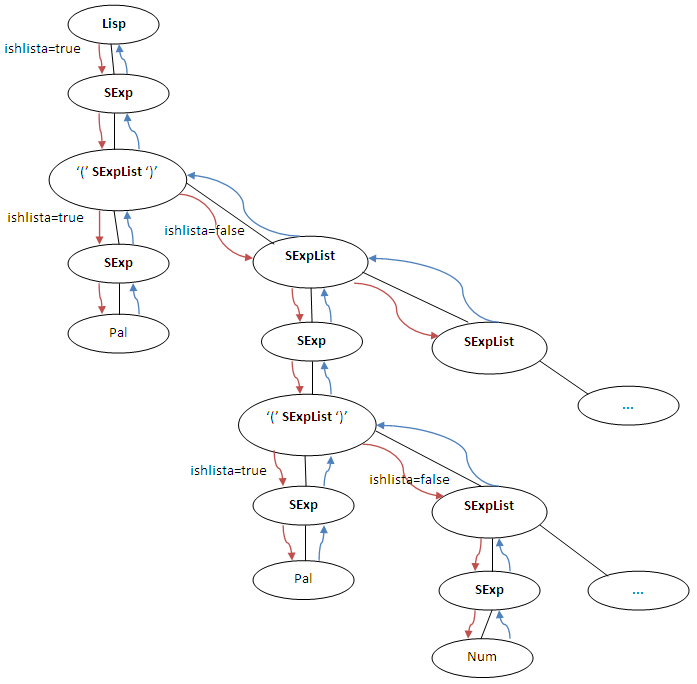
\includegraphics [width=0.7\textwidth] {stuff/diagrama.png}
\caption{Árvore de derivação da linguagem Lisp}\label{fig arv}
\end{center}
\end{figure}

O segundo valor, \emph{operandos}, é um atributo sintetizado do tipo \emph{[String]}. Nas produções \texttt{SExp --> num} e \texttt{SExp --> pal} será confirmado se se trata do primeiro elemento de uma lista. Caso seja, será retornado uma lista com o valor correspondente, caso contrário, será retornado uma lista vazia, para posteriormente ser concatenado com os outros valores lidos (código em ~\ref{lst_semantics2}).\\

\begin{lstlisting}[frame=single, numbers=right, basicstyle=\tiny, caption={Parte do código onde se verifica se é o primeiro elemento da lista}, label={lst_semantics2}]
se::SExp ::= pl::Pal
{se.output="palavra";
se.operandos = if se.ishlista then [pl.lexeme] else [] ;
}
\end{lstlisting}

\subsection{Alínea c) e d)}

Estas duas alíneas ainda não foram devidamente resolvidas por falta de exploração da ferramenta \emph{Silver}. Mas, do ponto visto teórico, a resolução passava por criar um atributo herdado que tivesse a estrutura de uma lista (para a alínea \emph{c)}).

\begin{lstlisting}[frame=single, numbers=right, basicstyle=\tiny, caption={Parte do código onde se define o atributo biblioteca}, label={lst lisp}]
synthesized attribute biblioteca :: [String];
attribute biblioteca occurs on Lisp,SExp,SExpList;
\end{lstlisting}

Este atributo seria a biblioteca de operandos, criado na produção inicial (como se pode ver em~\ref{lst lisp2}), e deveria descer na árvore de derivação até à leitura dos operandos para se verificar se o valor seria correcto ou não. A ferramenta \emph{Silver} dispõe de várias funções para trabalhar com listas. A função \emph{listContains} seria a ideal para resolver esta alínea, mas infelizmente não se a conseguiu utilizar.

\begin{lstlisting}[frame=single, numbers=right, basicstyle=\tiny, caption={Parte do código para a criação da biblioteca}, label={lst lisp2}]
concrete production program
ls::Lisp ::= se::SExp
{
ls.biblioteca = ["add"] ++ ["mul"] ++ ["let"];
se.biblioteca = ls.biblioteca;
}
\end{lstlisting}

Para a alínea \emph{d)}, a solução passaria por criar uma estrutura mais complexa da biblioteca que indicasse a cada operador o número correspondente de argumentos.

\end{document}
